\documentclass{beamer}
\usepackage{tikz}

\usetikzlibrary{positioning,shapes,shadows,arrows}

\mode<presentation>
{
 \usetheme{Warsaw}
}
\title{Powersaving Disk Arrays}
\subtitle{Raspberry PI as simple "Wake Up" server}
\date[2014]{OSS Weekend 2014}
\author[R. Strobl]{Radoslav Strobl}

\begin{document}

\frame{\maketitle} %

\begin{frame}{Overview}
    \begin{itemize}
        \vfill\item Requirements
        \vfill\item Basic Scheme
        \vfill\item How it works
        \vfill\item Limitations
    \end{itemize}
\end{frame}

\begin{frame}{Requirements}
    \begin{itemize}

            \item<1-> Raspebrry PI Model B (Or other Low-power board with ethernet)
                \begin{itemize}
                    \item Linux
                    \item libcap (http://www.tcpdump.org/)
                    \item psdad daemon (https://github.com/takada07/psdad)
                    \item iptables
                \end{itemize}
            \item<2-> Power Management capable machine
                \begin{itemize}
                    \item Supports suspend to RAM
                    \item Supports WOL (Wake on LAN)
                \end{itemize}
            \item<3-> Switch/Router
            \item<4-> Client machine (Laptop, Phone, Tablet, PC, etc...)
    \end{itemize}
\end{frame}

\begin{frame}{Basic Scheme}
\begin{tikzpicture}
    \node[inner sep=0pt] (laptop) at (0,3)
        {
\includegraphics[width=.25\textwidth]{img/laptop.png}};
    \node[inner sep=0pt] (desktop-on) at (8,3)
        {
\includegraphics[width=.25\textwidth]{img/desktop-on.png}};
        \node[color=white] (suspend) at (8,5) {SUSPEND};
    \node[inner sep=0pt] (raspi) at (4,3)
        {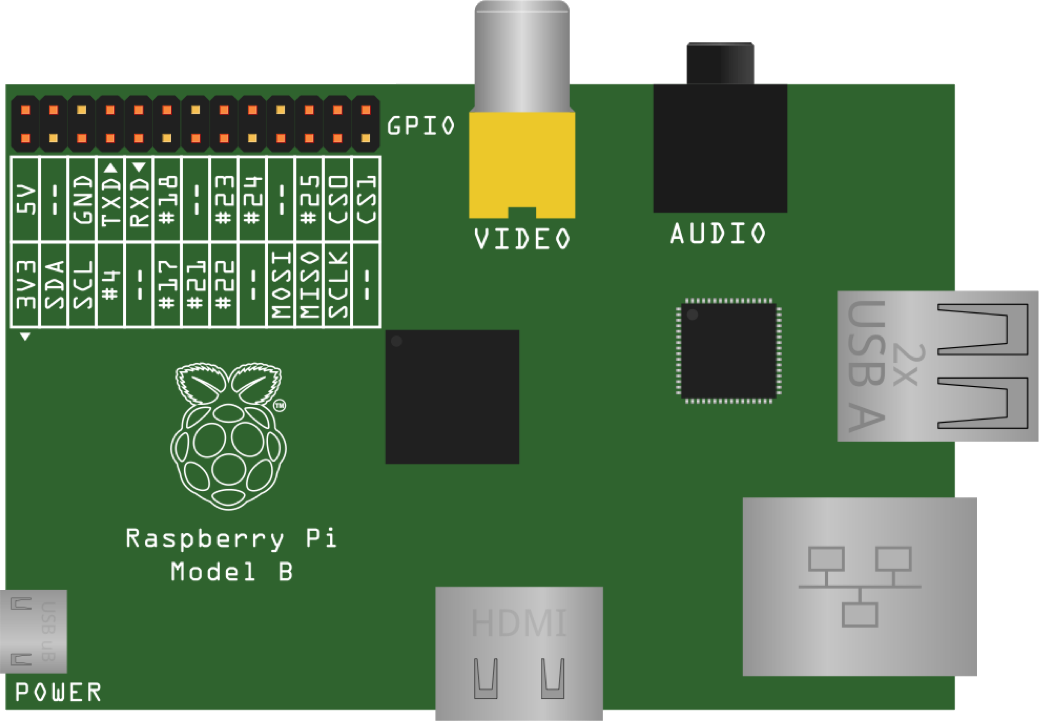
\includegraphics[width=.125\textwidth]{img/raspi.png}};
    \node[color=white] (filterrst) at (4,4) {Filter (RST,ACK)};        
    \node[inner sep=0pt] (switch) at (4,0)
        {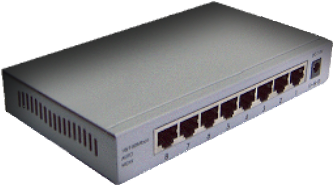
\includegraphics[width=.25\textwidth]{img/switch.png}};
    \draw (0,2) -- (0,-0.2)
            node[near start,fill=white] {eth0 192.168.10.102} -- (2.5,-0.2);
    \draw (5.5,-0.2) -- (8,-0.2) -- (8,1.7)
            node[near end, fill=white] {eth0 192.168.10.100};
    \draw (4,2.4) -- (4,0.7)
        node[near start, fill=white] {eth0 192.168.10.101};
\end{tikzpicture}
\end{frame}

\begin{frame}{How it Works}
\begin{tikzpicture}
    \node[inner sep=0pt] (laptop) at (0,3)
        {
\includegraphics[width=.25\textwidth]{img/laptop.png}};
    \node[inner sep=0pt] (desktop-on) at (8,3)
        {
\includegraphics[width=.25\textwidth]{img/desktop-suspend.png}};
        \node [color=red] (suspend) at (8,5) {SUSPEND};
    \node[inner sep=0pt] (raspi) at (4,3)
        {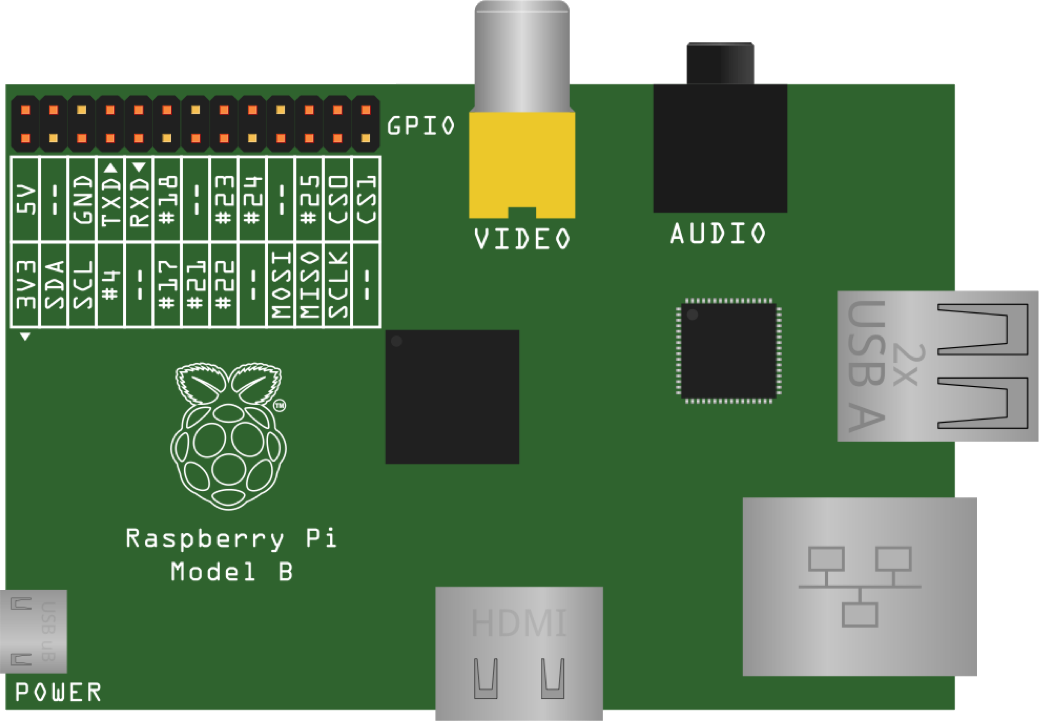
\includegraphics[width=.125\textwidth]{img/raspi.png}};
    \node[color=white] (filterrst) at (4,4) {Filter (RST,ACK)};        
    \node[inner sep=0pt] (switch) at (4,0)
        {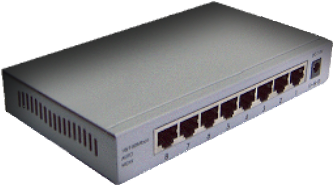
\includegraphics[width=.25\textwidth]{img/switch.png}};
    \draw (0,2) -- (0,-0.2)
            node[near start,fill=white] {eth0 192.168.10.102} -- (2.5,-0.2);
    \draw (5.5,-0.2) -- (8,-0.2) -- (8,1.7);
    \draw (4,2.4) -- (4,0.7)
        node[near start, fill=white] {eth0 192.168.10.101};
    \pause
    \draw [color=red] (4.1,2.4) -- (4.1,0.7)  -- (8.1,0.7) node[midway, fill=white]{PING} -- (8.1,1.7);
\end{tikzpicture}
\end{frame}

\begin{frame}{How it Works}
\begin{tikzpicture}
    \node[inner sep=0pt] (laptop) at (0,3)
        {
\includegraphics[width=.25\textwidth]{img/laptop.png}};
    \node[inner sep=0pt] (desktop-on) at (8,3)
        {
\includegraphics[width=.25\textwidth]{img/desktop-suspend.png}};
        \node [color=white] (suspend) at (8,5) {SUSPEND};
    \node[color=white] (filterrst) at (4,4) {Filter (RST,ACK)};
    \node[inner sep=0pt] (raspi) at (4,3)
        {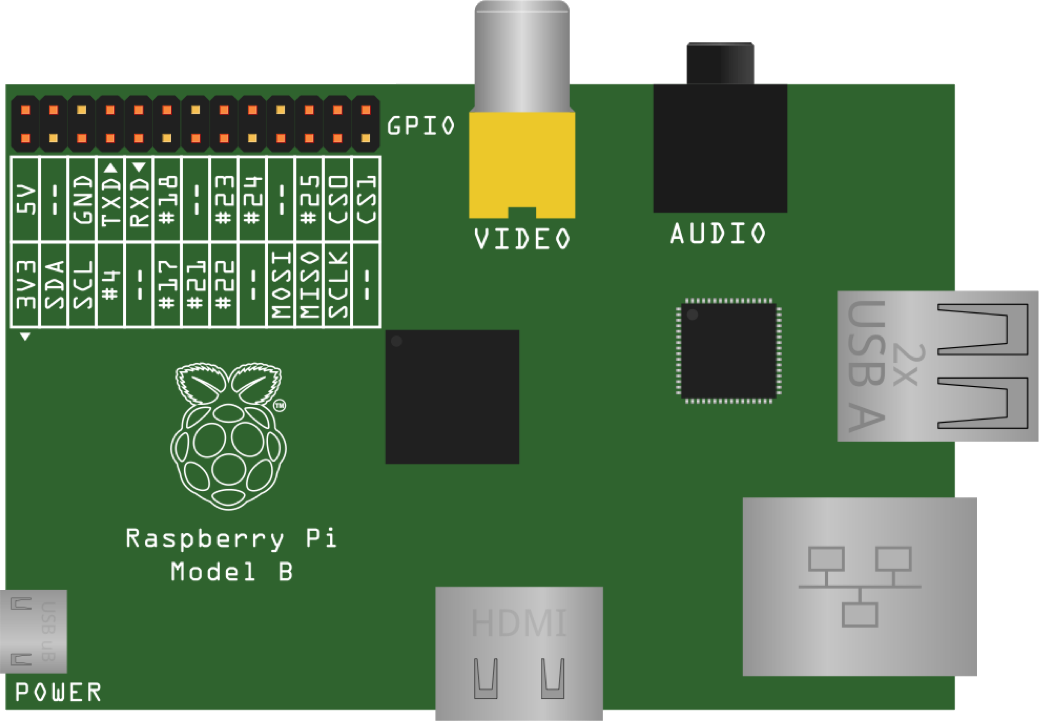
\includegraphics[width=.125\textwidth]{img/raspi.png}};
    \node[inner sep=0pt] (switch) at (4,0)
        {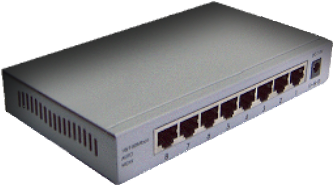
\includegraphics[width=.25\textwidth]{img/switch.png}};
    \draw (0,2) -- (0,-0.2)
            node[near start,fill=white] {eth0 192.168.10.102} -- (2.5,-0.2);
    \draw (5.5,-0.2) -- (8,-0.2) -- (8,1.7);
    \draw (4,2.4) -- (4,0.7)
        node[near start, fill=white] 
        {\begin{tabular}{cc}
            eth0 192.168.10.101 \\
            eth0:1 192.168.10.100 \\
        \end{tabular}};
\end{tikzpicture}
\end{frame}

\begin{frame}{And here comes the magic....}
\begin{tikzpicture}
    \node[inner sep=0pt] (laptop) at (0,3)
        {
\includegraphics[width=.25\textwidth]{img/laptop.png}};
    \node[inner sep=0pt] (desktop-on) at (8,3)
        {
\includegraphics[width=.25\textwidth]{img/desktop-suspend.png}};
    \node [color=white] (suspend) at (8,5) {SUSPEND};
    \node[inner sep=0pt] (raspi) at (4,3)
        {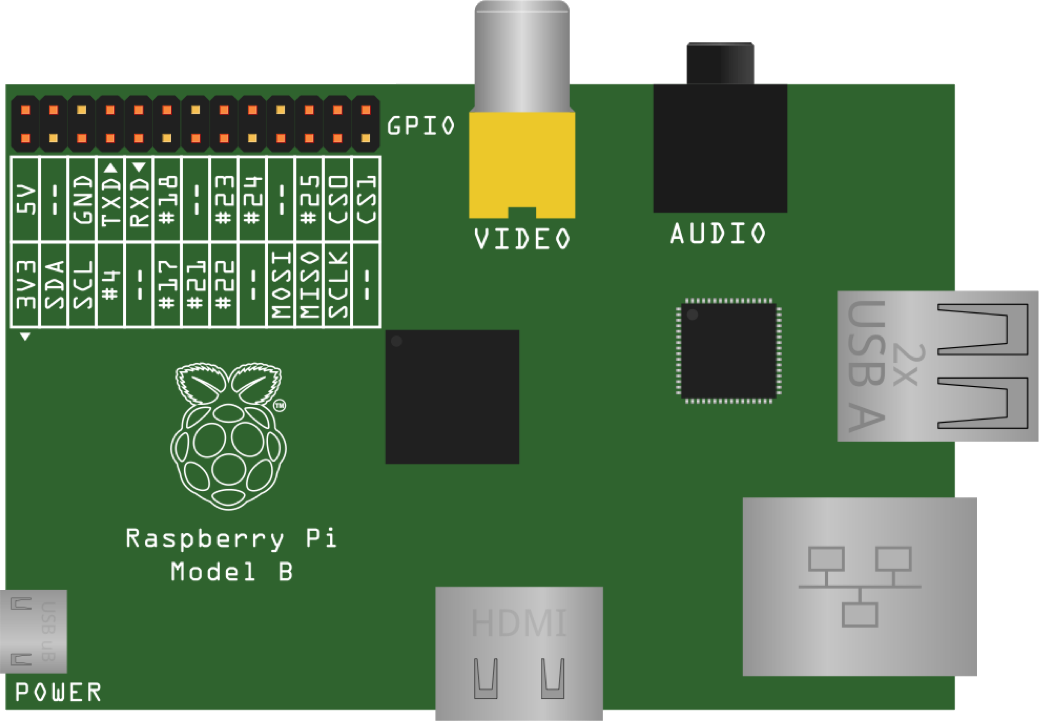
\includegraphics[width=.125\textwidth]{img/raspi.png}};
    \node[color=white] (filterrst) at (4,4) {Filter (RST,ACK)};
    \node[inner sep=0pt] (switch) at (4,0)
        {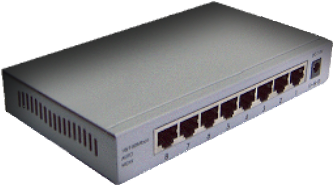
\includegraphics[width=.25\textwidth]{img/switch.png}};
    \draw (0,2) -- (0,-0.2)
            node[near start,fill=white] {eth0 192.168.10.102} -- (2.5,-0.2);
    \draw (5.5,-0.2) -- (8,-0.2) -- (8,1.7);
    \draw (4,2.4) -- (4,0.7)
        node[near start, fill=white] 
        {\begin{tabular}{cc}
            eth0 192.168.10.101 \\
            eth0:1 192.168.10.100 \\
        \end{tabular}};
    \pause
    \draw [->,color=blue,thick] (0.1,2) -- (0.1, -0.3) node[midway, fill=white] {req 192.168.10.100} -- (2.6, -0.3);
    \pause 
    \draw [->,color=blue,thick] (4.1,0.8) -- (4.1,1.5);
\end{tikzpicture}
\end{frame}

\begin{frame}{And here comes the magic....}
\begin{tikzpicture}
    \node[inner sep=0pt] (laptop) at (0,3)
        {
\includegraphics[width=.25\textwidth]{img/laptop.png}};
    \node[inner sep=0pt] (desktop-on) at (8,3)
        {
\includegraphics[width=.25\textwidth]{img/desktop-suspend.png}};
    \node [color=white] (suspend) at (8,5) {SUSPEND};
    \node[inner sep=0pt] (raspi) at (4,3)
        {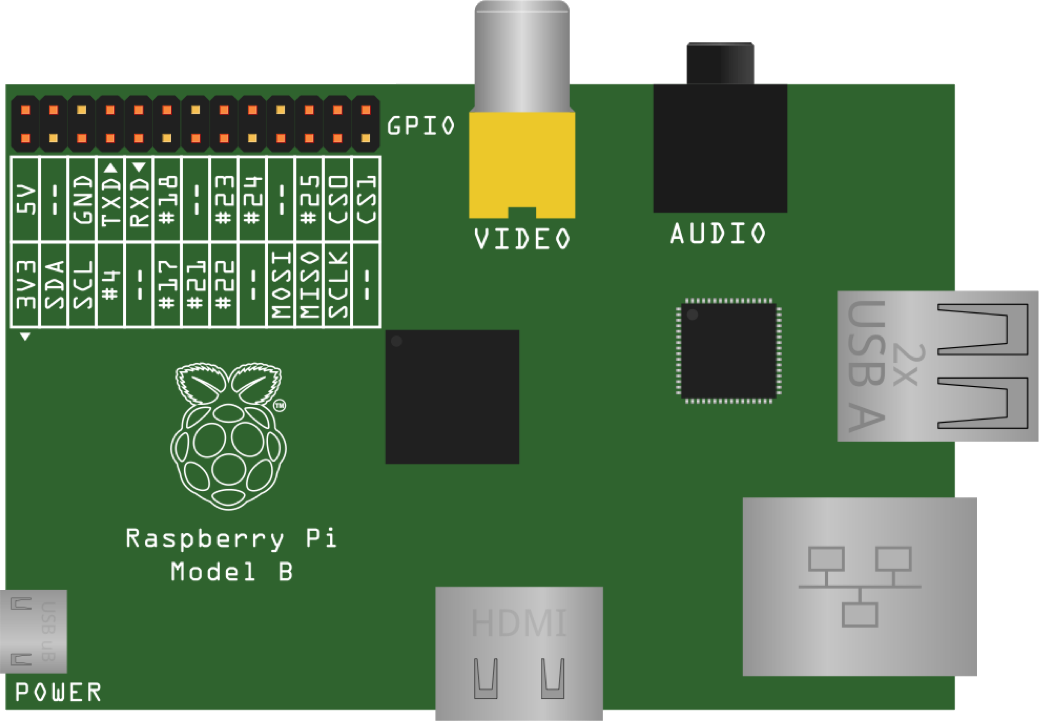
\includegraphics[width=.125\textwidth]{img/raspi.png}};
    \node[color=red] (filterrst) at (4,4) {Filter (RST,ACK)};
    \node[inner sep=0pt] (switch) at (4,0)
        {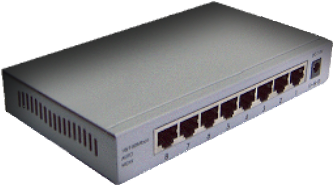
\includegraphics[width=.25\textwidth]{img/switch.png}};
    \draw (0,2) -- (0,-0.2)
            node[near start,fill=white] {eth0 192.168.10.102} -- (2.5,-0.2);
    \draw (5.5,-0.2) -- (8,-0.2) -- (8,1.7);
    \draw (4,2.4) -- (4,0.7)
        node[near start, fill=white] 
        {\begin{tabular}{cc}
            eth0 192.168.10.101 \\
            eth0:1 192.168.10.100 \\
        \end{tabular}};
    \draw [->,color=blue,thick] (0.1,2) -- (0.1, -0.3) node[midway, fill=white] {req 192.168.10.100} -- (2.6, -0.3);
    \draw [->,color=blue,thick] (4.1,0.8) -- (4.1,1.5);
\end{tikzpicture}
\end{frame}

\begin{frame}{And here comes the magic....}
\begin{tikzpicture}
    \node[inner sep=0pt] (laptop) at (0,3)
        {
\includegraphics[width=.25\textwidth]{img/laptop.png}};
    \node[inner sep=0pt] (desktop-on) at (8,3)
        {
\includegraphics[width=.25\textwidth]{img/desktop-suspend.png}};
    \node [color=white] (suspend) at (8,5) {SUSPEND};
    \node[inner sep=0pt] (raspi) at (4,3)
        {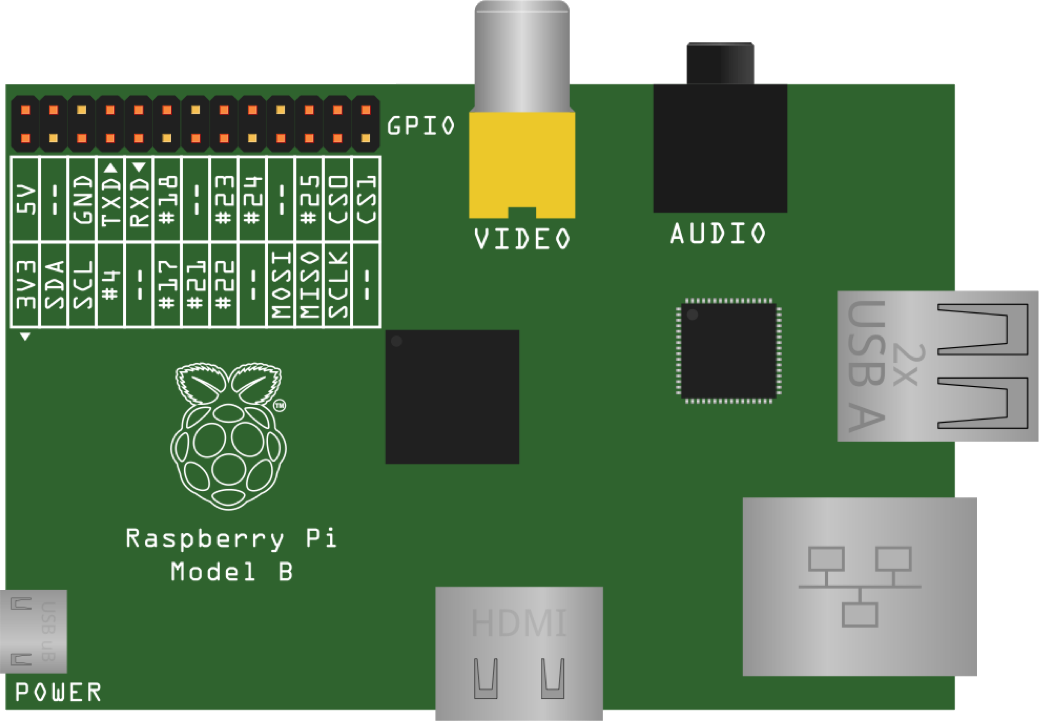
\includegraphics[width=.125\textwidth]{img/raspi.png}};
    \node[color=white] (filterrst) at (4,4) {Filter (RST,ACK)};
    \node[inner sep=0pt] (switch) at (4,0)
        {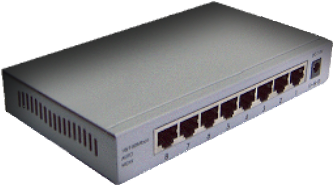
\includegraphics[width=.25\textwidth]{img/switch.png}};
    \draw (0,2) -- (0,-0.2)
            node[near start,fill=white] {eth0 192.168.10.102} -- (2.5,-0.2);
    \draw (5.5,-0.2) -- (8,-0.2) -- (8,1.7);
    \draw (4,2.4) -- (4,0.7)
        node[near start, fill=white] 
        {eth0 192.168.10.101};
    \draw [->,color=blue,thick] (0.1,2) -- (0.1, -0.3) node[midway, fill=white] {req 192.168.10.100} -- (2.6, -0.3);
    \pause
    \draw [->,color=green] (4.1,2.4) -- (4.1,0.7)  -- (8.1,0.7) node[midway, fill=white]{Wake on Lan} -- (8.1,1.7);    
\end{tikzpicture}
\end{frame}

\begin{frame}{And here comes the magic....}
\begin{tikzpicture}
    \node[inner sep=0pt] (laptop) at (0,3)
        {
\includegraphics[width=.25\textwidth]{img/laptop.png}};
    \node[inner sep=0pt] (desktop-on) at (8,3)
        {
\includegraphics[width=.25\textwidth]{img/desktop-on.png}};
    \node [color=green] (suspend) at (8,5) {WAKE UP};
    \node[inner sep=0pt] (raspi) at (4,3)
        {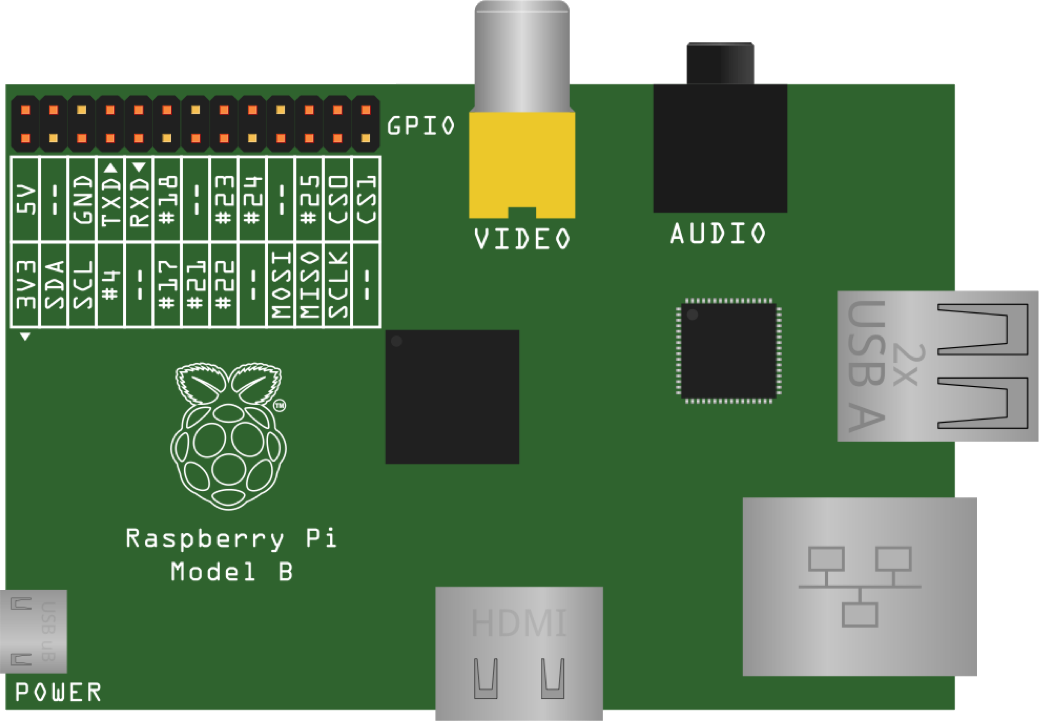
\includegraphics[width=.125\textwidth]{img/raspi.png}};
    \node[color=white] (filterrst) at (4,4) {Filter (RST,ACK)};
    \node[inner sep=0pt] (switch) at (4,0)
        {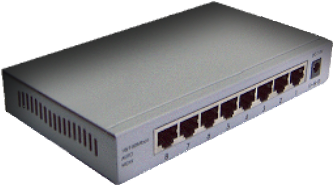
\includegraphics[width=.25\textwidth]{img/switch.png}};
    \draw (0,2) -- (0,-0.2)
            node[near start,fill=white] {eth0 192.168.10.102} -- (2.5,-0.2);
    \draw (5.5,-0.2) -- (8,-0.2) -- (8,1.7);
    \draw (4,2.4) -- (4,0.7)
        node[near start, fill=white] 
        {eth0 192.168.10.101};
    \draw [->,color=blue,thick] (0.1,2) -- (0.1, -0.3) node[midway, fill=white] {req 192.168.10.100} -- (2.6, -0.3);
    \draw [->,color=green] (4.1,2.4) -- (4.1,0.7)  -- (8.1,0.7) node[midway, fill=white]{Wake on Lan} -- (8.1,1.7);    
\end{tikzpicture}
\end{frame}

\begin{frame}{And here comes the magic....}
\begin{tikzpicture}
    \node[inner sep=0pt] (laptop) at (0,3)
        {
\includegraphics[width=.25\textwidth]{img/laptop.png}};
    \node[inner sep=0pt] (desktop-on) at (8,3)
        {
\includegraphics[width=.25\textwidth]{img/desktop-on.png}};
    \node [color=white] (suspend) at (8,5) {WAKE UP};
    \node[inner sep=0pt] (raspi) at (4,3)
        {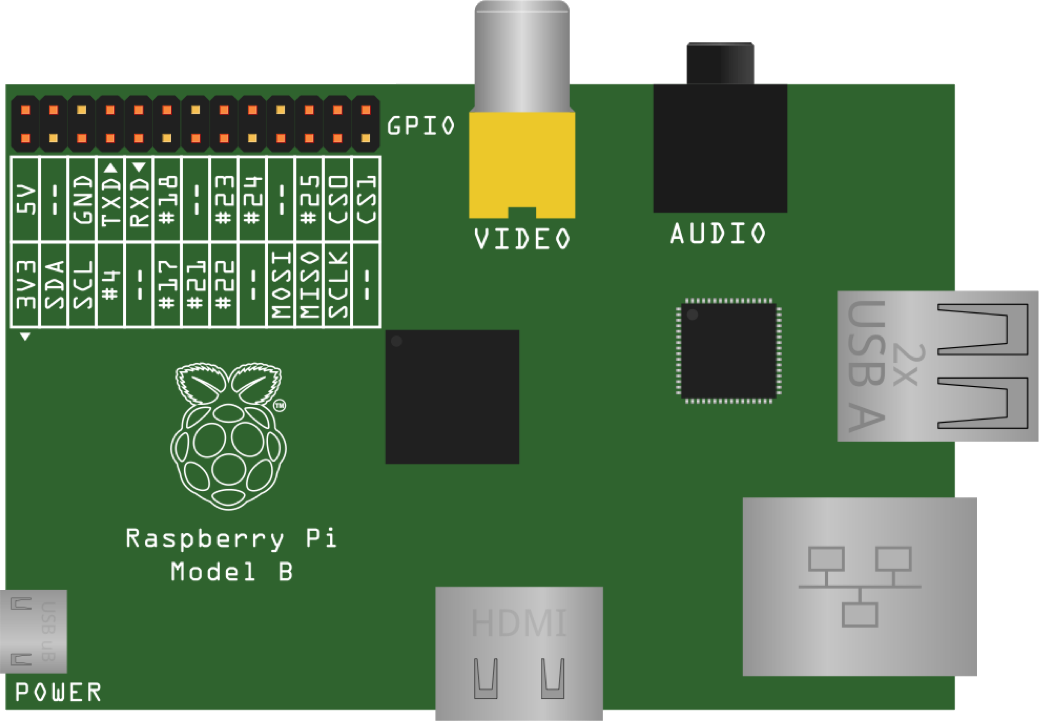
\includegraphics[width=.125\textwidth]{img/raspi.png}};
    \node[color=white] (filterrst) at (4,4) {Filter (RST,ACK)};
    \node[inner sep=0pt] (switch) at (4,0)
        {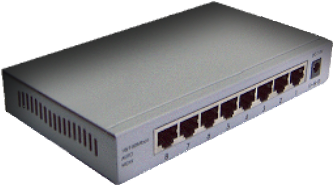
\includegraphics[width=.25\textwidth]{img/switch.png}};
    \draw (0,2) -- (0,-0.2)
            node[near start,fill=white] {eth0 192.168.10.102} -- (2.5,-0.2);
    \draw (5.5,-0.2) -- (8,-0.2) -- (8,1.7)
            node[near end, fill=white] {eth0 192.168.10.100};
    \draw (4,2.4) -- (4,0.7)
        node[near start, fill=white] 
        {eth0 192.168.10.101};
    \draw [->,color=blue,thick] (0.1,2) -- (0.1, -0.3) node[midway, fill=white] {req 192.168.10.100} -- (2.6, -0.3);
    \pause
    \draw [->,color=blue,thick] (5.4, -0.3) -- (8.1,-0.3) -- (8.1,1.6);
\end{tikzpicture}
\end{frame}

\begin{frame}{And here comes the magic}
    How it looks real (video)
\end{frame}

\begin{frame}{Limitations}
    \begin{itemize}
        \item<1-> Static IP (can not use DHCP on router)
        \item<2-> Currently only TCP connections are supported
        \item<3-> No samba support (Samba is very talkative protocol)
        \item<4-> Slow responses (refresh ARP cache?, long timeout for TCP retransmission)
    \end{itemize}
\end{frame}

\begin{frame} {Thanks}
    \center {God bless you all}
\end{frame}
\end{document}
